\section{Kode dan Implementasi}
Perintah navigasi direktori Android
\lstinputlisting{src/api/config.php}
\lstinputlisting{src/api/conn.php}

\lstinputlisting{src/api/mahasiswa/mahasiswa_login.php}
\lstinputlisting{src/api/mahasiswa/mahasiswa_registrasi.php}
\lstinputlisting{src/api/mahasiswa/mahasiswa_absensi.php}
\lstinputlisting{src/api/mahasiswa/mahasiswa_kegiatan.php}
\lstinputlisting{src/api/mahasiswa/mahasiswa_notifikasi.php}
\lstinputlisting{src/api/mahasiswa/mahasiswa_pembimbing.php}
\lstinputlisting{src/api/mahasiswa/mahasiswa_perusahaan.php}
\lstinputlisting{src/api/mahasiswa/mahasiswa_progress.php}
\lstinputlisting{src/api/mahasiswa/mahasiswa_progress_harian.php}
\lstinputlisting{src/api/mahasiswa/mahasiswa_ubah.php}
\lstinputlisting{src/api/mahasiswa/mahasiswa.php}

\lstinputlisting{src/api/dosen/dosen_login.php}
\lstinputlisting{src/api/dosen/dosen_mahasiswa.php}
\lstinputlisting{src/api/dosen/dosen_notifikasi.php}
\lstinputlisting{src/api/dosen/dosen_progress.php}
\lstinputlisting{src/api/dosen/dosen_progress_harian.php}
\lstinputlisting{src/api/dosen/dosen_ubah.php}
\lstinputlisting{src/api/dosen/dosen.php}

\section{Web}
\subsection{Dapur Hosting}
Di tutorial kali ini kita akan menggunakan jasa web hosting. Web hosting adalah layanan penyimpanan file website, email, dan database yang terkoneksi ke internet dan dapat diakses dengan nama domain. Dapur Hosting menyediakan 2 pilihan lokasi web hosting murah, yaitu di Indonesia dan USA
\begin{itemize}
	\item Siapkan file yang akan di upload
	\begin{enumerate}
\begin{figure}[H]
	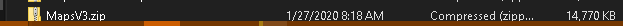
\includegraphics[width=8cm]{figures/web/1_fileupload.PNG}
	\centering
	\caption{Upload.}
\end{figure}	
	\item Login ke dapurhosting
\begin{figure}[H]
	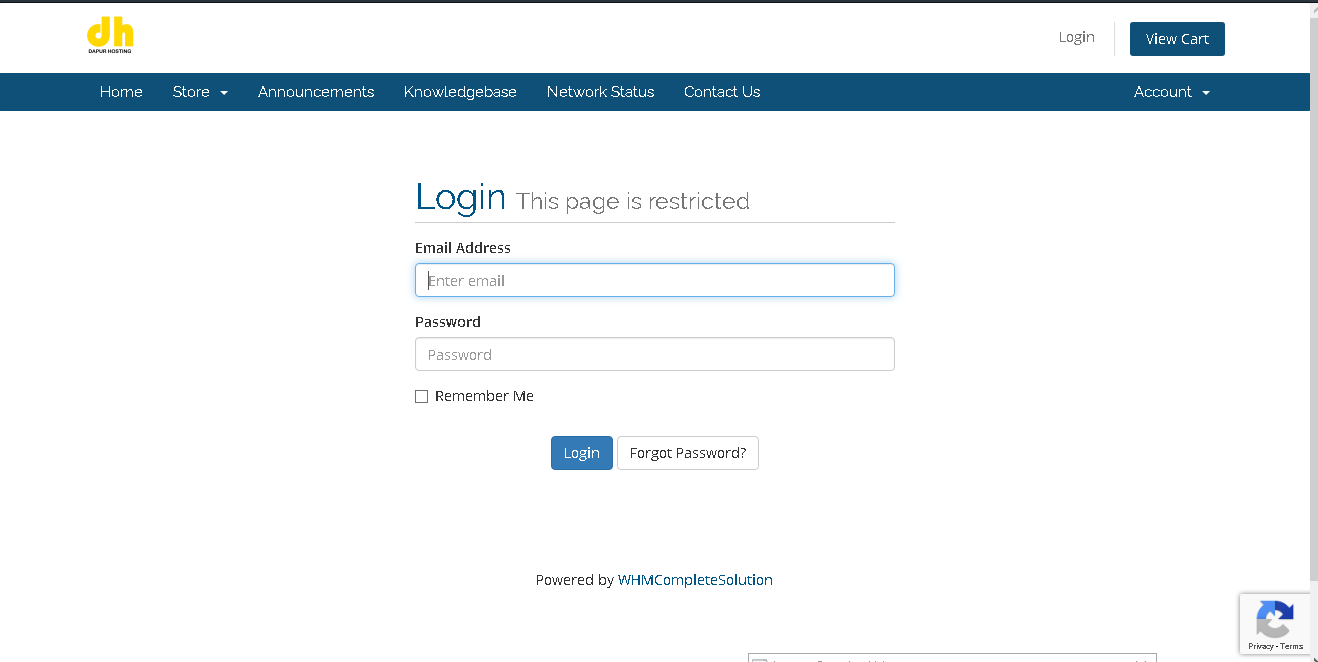
\includegraphics[width=8cm]{figures/web/2_logindapurhosting.PNG}
	\centering
	\caption{Login.}
\end{figure}	

	\item masuk ke file manager dan upload disini
\begin{figure}[H]
	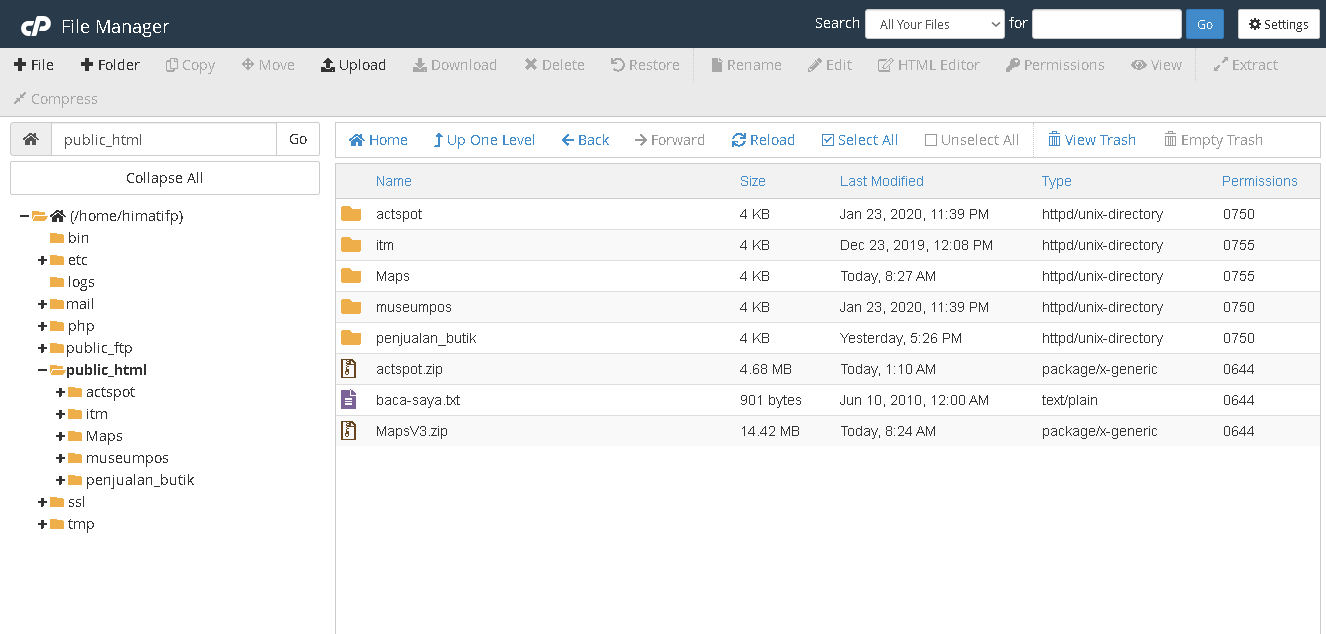
\includegraphics[width=8cm]{figures/web/3_filemanager.PNG}
	\centering
	\caption{Upload file.}
\end{figure}	
	
	\item Setting config database.php
\begin{figure}[H]
	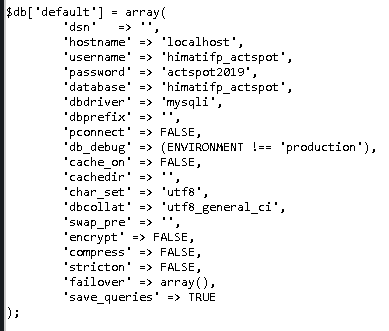
\includegraphics[width=8cm]{figures/web/4_databasesetting.PNG}
	\centering
	\caption{database file.}
\end{figure}	
	\item setting config .php
\begin{figure}[H]
	
\includegraphics[width=8cm]{figures/web/5_config.PNG}
	\centering
	\caption{config file.}
\end{figure}	

	\item Hasil
\begin{figure}[H]
	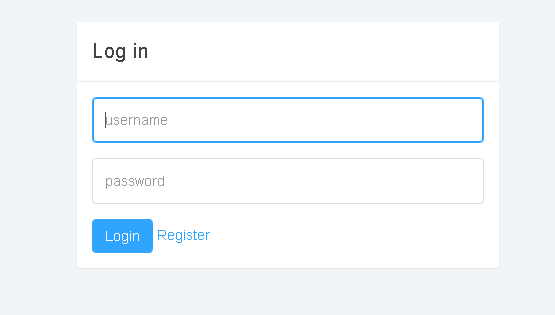
\includegraphics[width=8cm]{figures/web/6_tampilan.PNG}
	\centering
	\caption{Tampilan}
\end{figure}	
	\end{enumerate}
\end{itemize}


Source code web
\lstinputlisting{src/web/config/config.php}
\lstinputlisting{src/web/config/database.php}

\lstinputlisting{src/web/controllers/ckelolauser.php}
\lstinputlisting{src/web/controllers/clogin.php}
\UseRawInputEncoding{src/web/controllers/cregister.php}
\lstinputlisting{src/web/controllers/dashboard.php}

\lstinputlisting{src/web/models/mdatapeta.php}
\lstinputlisting{src/web/models/mdatauser.php}
\lstinputlisting{src/web/models/mlogin.php}
\lstinputlisting{src/web/models/mregister.php}

\lstinputlisting{src/web/views/chartview.php}
\lstinputlisting{src/web/views/dosen.php}
\lstinputlisting{src/web/views/index.php}
\lstinputlisting{src/web/views/login.php}
\lstinputlisting{src/web/views/vgrafik.php}
\lstinputlisting{src/web/views/vkelolauser.php}
\lstinputlisting{src/web/views/vregister.php}




